\section{Real World Languages}
\label{sec:real}

In the introduction, we stated that the original motivation behind
this work was to formally specify a
coarse-grained information flow control language for JavaScript.
%
Indeed, our formalism serves as the theoretical foundation for two
IFC systems for JavaScript, built on top of Node.js as well as
the web browser engine Gecko.

In this section, we describe these two implementations.  Furthermore,
we consider how our formalism could be applied to the C programming
language and connect it to a previous IFC system for Haskell.
%
The goal of this section is to show the flexibility of the embedding in settings with
vastly different properties and discuss the
semantic gap that must be overcome to apply our formalism
to other systems.
%
%% Two of the systems we describe have been implemented: the Haskell
%% system~\cite{lio} and the COWL~\cite{swapi} system; we leave the
%% implementation of the IFC system for C to future work.


\subsection{JavaScript}
\label{sec:real:js}

JavaScript, as specified by
ECMAScript~\cite{ecma}, does not have any built-in
functionality for I/O.
%(we denote this language as |targetLangJS|).
%
For this language, which we denote by |targetLangJS|, the IFC system
|specLangJS roundrobinf| can be implemented by exposing IFC primitives
to JavaScript as part of the runtime, and running multiple instances
of the JavaScript virtual machine in separate OS-level threads.
%
Unfortunately, this becomes very costly when an application relies on
many tasks.
%
For instance, consider a server-side web application that
creates a new task for each HTTP request.  The overhead would
quickly become impractical.

However, this issue of performance and JavaScript isolation is not
unique to our work and has been solved by browser engines,
which also
rely on the isolation of content from
different origins (e.g., two iframes of different origins) to
implement the same-origin policy.
%
Since creating an OS thread for each iframe is expensive, both
Google's V8 and Mozilla's SpiderMonkey provide a means for running
JavaScript code in isolation in a single OS thread,
on disjoint sub-heaps.
%
In V8, this unit of isolation is called a \emph{context}; in
SpiderMonkey, it is called a \emph{compartment}.
%
Each context/compartment is associated with a global object, which, by
default, implements the JavaScript standard library (e.g.,
\verb|Object|, \verb|Array|, etc.).
%
Naturally, our notion of a task for JavaScript directly corresponds to
a context/compartment.


When JavaScript is embedded in web browser engines, such as Google's
Blink or Mozilla's Gecko, or in server-side platforms such as Node.js,
additional APIs such as the Document Object Model (DOM) or the file
system get exposed as part of the runtime system.
These features are exposed by extending the global object, just like
for the standard library.  For this reason, it is easy to modify
these systems to remove arbitrary external effects when implementing
an IFC system so important effects can be reintroduced in a safe manner.


\subsubsection{Server-side embedding: Node.js}

We have implemented |specLangJS seqf| for Node.js in the form of a module
(library), which does not modify the Node.js or V8 code-base in any
way.
%
Our implementation provides a library for creating new tasks, i.e.,
contexts whose global object only contains the standard JavaScript
library as well as our IFC primitives (such as |send| and |sandbox|).
%
In turn, these tasks can create new tasks with |sandbox|.
%
In our formal treatement, |sandbox| is defined with |ap klone tS = tS0|,
where |tS0| is the global object corresponding to the standard
JavaScript library and our IFC primitives.
 
\begin{figure}
\centerline{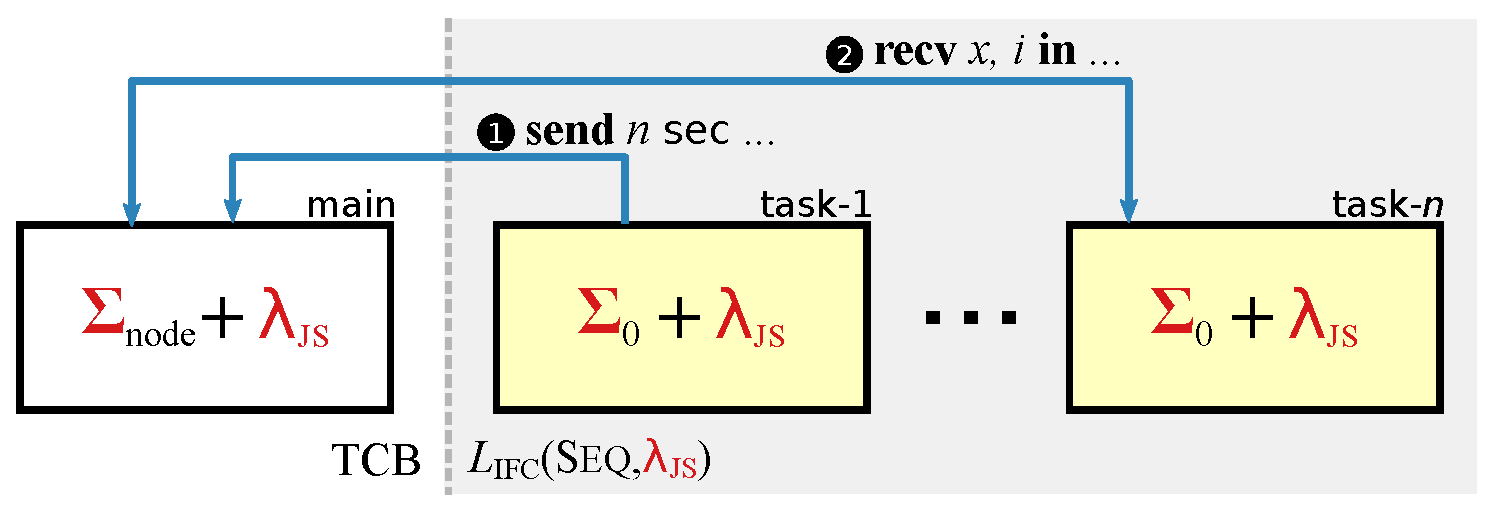
\includegraphics[width=\columnwidth]{figs/node}}
\caption{\label{fig:node} Retrofitting Node.js JavaScript with IFC.
This example shows how our trusted monitor (left) is used to mediate
communication between two tasks for which IFC is enforced (right).}
\end{figure}
%
All IFC primitives are mediated by the trusted library code (executing
as the main Node.js context), which tracks the current label, messages,
etc.\ of each task.  An example for |send|/|recv| is shown in
Figure~\ref{fig:node}.
%While V8 provides a means for sharing any object between contexts (used
%by same-origin contexts in Blink),
Our system conservatively restricts
the kinds of messages that can be exchanged by tasks by
only allowing string values to be exchanged via |send| (and |sandbox|).
%
In our formalization, this amounts to restricting the IFC language rule
for |send| in the following way:
%{
\newcommand{\str}{"string"}
%format tOf (e) = "\texttt{typeOf}("e")\texttt{ === \str}"
%format ttrue = "\texttt{true}"
\begin{mathpar}
\inferrule[JS-send]
{
|il canFlowTo il'|\\
|iS(id') = Q|\\
|iS' = iS [ mapsto id' (il', id,  iv) , Q ]|\\
|ie = IT te|\\
|conf tS (tOf te) -> conf tS ttrue|
}
{|
iconf iS (fullconf id il tS (iniEi (send id' il' iv)), ldots)
.->
iS'; sched step (fullconf id il tS (iniEi unit), ldots)
|}
\end{mathpar}
%}
%
For convenience, we have implemented a library that provides
more flexible primitives, which, among other things,
automatically marshalls JSON objects to/from strings on each
|send|/|recv|.

While the described system implements |specLangJS seqf|, server-side
applications may require access to the file system, HTTP server, HTTP
client, etc.
%
Unfortunately, our formalism does not capture such external effects
and exposing the Node.js libraries directly to sandboxed tasks is unsafe.
%
We, instead, implement libraries such as a labeled file system as
message exchanges between the sandboxed tasks (e.g., \textsf{task-1}
in Figure~\ref{fig:node}) and the main Node.js task that implements
our IFC monitor.\footnote{
  Importantly, we provide mostly-identical interfaces to
  the standard Node.js libraries, hiding the underlying
  message-passing implementations.
}
%
(This is safer than the approach of simply wrapping objects, which can
potentially allow objects to be accessed outside the context.)
%
This task is trusted to ensures that labels are
propagated to files and the labels of the task and the file in question permit
this flow.
%
Unfortunately, while imposing such a proof burden on the
framework developer is undesirable, this is also somewhat expected:
different language environments expose different libraries for
handling external I/O.
%
For instance, in the case of Node.js, how labels interact with the
file system may even vary according to the application (e.g.,
in the IFC system Hails~\cite{hails}, labels are not persisted).
%
While we can extend our formalism to model a particular interface to
the file system, HTTP client, etc. the utility of this formalization is
unclear and left to future work.
%


\subsubsection{Client-side embedding: Gecko}

We now describe some of the implementation aspects of
COWL~\cite{swapi}, for which this work serves as the theoretical
underpinning.
%
Since the architecture of COWL is similar to that of Node.js, we focus
on the main differences.
 
Tasks in COWL usually correspond to browsing contexts, such as iframes,
where the global object |tS0| also contains the DOM, the
\verb|XMLHttpRequest| (XHR) object, etc.
%
Existing browser APIs also offer \emph{web workers}, which can
be spawned by JavaScript code and have
the same isolation properties as tasks in our system.
%
The isolation of web workers was motivated by the lack of multithreading
in JavaScript; however, their isolation properties are equally useful for information
flow control.

To ensure that JavaScript code cannot communicate using these objects
(e.g., to the network with XHR or persistent storage using the DOM),
COWL additionally uses content security policy (CSP)~\cite{csp1.1}.\footnote{
  Since CSP does not yet restrict message-passing or navigation, this
  was addressed explicitly.
}
%
Note, that this does not prevent tasks from manipulating the DOM
(e.g., to render information), so external effects due to DOM access
are also suppressed.
%
Simply disallowing all external effects for all browsing contexts is
overly-restricting; pages typically load images, perform XHR requests,
etc.
%
Hence, COWL allows
controlled network communication (inter-frame communication is
dictated by our |send| rule) by associating an implicit label with a
remote host: namely the label corresponding to its origin.
%
In turn, when a task perform a request, the COWL runtime performs the
same label check as that of |send|, e.g., does the task label flow to
the remote origin label.

Once again, while the external effects of COWL can be formally modeled,
we do not model these effects in our more general framework, since, like
for Node.js case, they are a platform-specific
detail.
%
Indeed, even the labeled HTTP client in  Node.js and COWL differ, even
though they're both JavaScript systems, simply because of the
differing environments.



\subsection{Haskell}
\label{sec:real:hs}
Our work borrows many ideas from the Haskell coarse-grained IFC
system LIO~\cite{lio, stefan:addressing-covert}.
%
LIO relies on Haskell's strong type system and monadic encoding of
side-effecting computations to achieve isolation and define the IFC
sub-language.
%
Specifically LIO provides the \verb|LIO| monad as a way of restricting
(almost all) side-effects; this monad also keeps track of a current
label which is, in turn, used by trusted code when defining core IFC
functions, such as |getLabel|.
%
In the context of our framework, LIO can be understood as follows: the
\emph{pure subset} of Haskell is the target language, while the
monadic subset of Haskell, operating in the \verb|LIO| monad, is the
IFC language.
 
Indeed, by rephrasing LIO in terms of our framework, we simplified
LIO's treatment of exceptions.
%
LIO originally associated labels with exceptions, in a
similar style to fine-grained
systems~\cite{stefan:2012:arxiv-flexible, Breeze}.
%
In particular, the label of an exception was set to the current label
at the time of the throw, and used by a custom catch construct to
raise the current label, thereby preventing leaks due exceptional
control flows.
%
In addition to being overly complex, the interaction of exceptions
with clearance (which sets an upper bound on the current label, see
Section~\ref{sec:extensions:clearance}) was incorrect: the clearance
was restored to the clearance at point of the catch (a consequence of
defining \verb|LIO| using a State monad).
%
Moreover, pure exceptions (e.g., divide by zero) always percolated to
trusted code, effectively allowing for denial of service attacks.
%
By using isolated tasks, and thus treating the current label (and
clearance) as global, the underlying Haskell exception system can be
used directly: exceptional control flow does not affect IFC.






\subsection{C}
\label{sec:real:c}
%
C programs are able to execute arbitrary (machine) code, access
arbitrary memory, and perform arbitrary system calls.
%
Thus, the confinement of C programs must be imposed by the underlying OS
and hardware.
%
For instance, this isolation can be achieved using Dune's hardware protection
mechanisms~\cite{Belay:2012:DSU:2387880.2387913}, similar to a simpler
version of Wedge~\cite{Belay:2012:DSU:2387880.2387913,
Bittau:2008:WSA:1387589.1387611} with an information flow control
policy.
%
Using page tables, a (trusted) IFC runtime could ensure that each task,
implemented as a lightweight process, can only access the memory it
allocates--tasks do not have access to any shared memory.
%
In addition, ring protection could be used to intercept system
calls performed by
a task and only permit those corresponding to our IFC language (such as
|getLabel| or |send|).
%
Dunes hardware protection mechanism allows us to provide a concrete
implementation that is efficient and relatively simple to reason
about, but other sandboxing mechanisms could be used in place of Dune.

In this setting, the combined language of Section~\ref{sec:retrofit}
can be interpreted in the following way: calling from the target
language to the IFC language corresponds to invoking a system call.
%
Creating a new task with the |sandbox| system call corresponds to
\emph{forking} a process.  Using page tables we can ensure that
there will be no shared memory
(effectively
defining |ap klone tS
= tS0|, where |tS0| is the set of pages necessary to bootstrap a
lightweight process.)
%
Similarly, control over page tables and protection bits allows us to
define a |send| syscall that copies pages to our
(trusted) runtime queue; and, correspondingly, a |recv| that copies
the pages from the runtime queue to the (untrusted) receiver.
%
Since C is not memory safe, conditions on these system calls are
meaningless.

We leave an actual implementation of an IFC system for C as
future work.
